\documentclass[amsmath, amssymb, aip, jmp, reprint]{revtex4-2}
\usepackage{tikz}
\usetikzlibrary{shapes.geometric}
\usetikzlibrary{decorations.markings}

\begin{document}

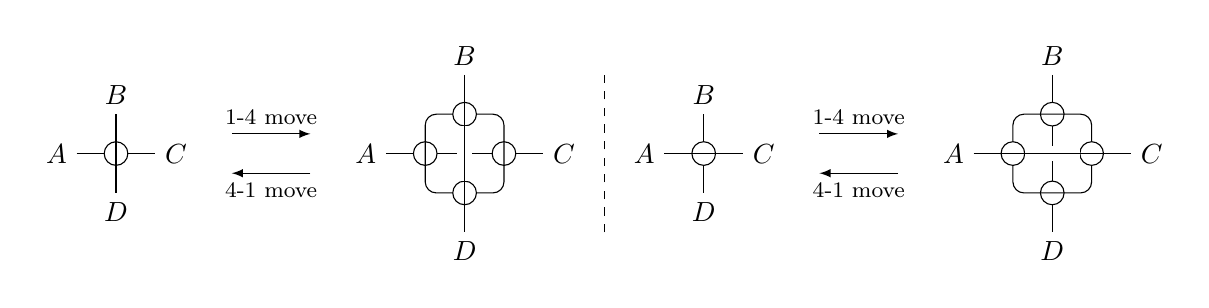
\begin{tikzpicture}[> = latex]
\matrix[column sep = 0.25 cm, row sep = 0.5 cm]{

	% Single vertex subgraph

	\draw (-0.5, 0) node [left] {$A$} -- (0.5, 0) node [right] {$C$};
	\draw [fill = white] (0, 0) circle (0.15);
	\draw (0, -0.5) node [below] {$D$} -- (0, 0.5) node [above] {$B$};

&

	\begin{scope}[->, font = \footnotesize]

		\draw (0, 0.25) -- node [above] {1-4 move} (1, 0.25);
		\draw (1, -0.25) -- node [below] {4-1 move} (0, -0.25);

	\end{scope}

&

	% 4-vertex subgraph

	\draw (-1, 0) node [left] {$A$} -- (1, 0) node [right] {$C$};

	\draw [fill = white] (-0.5, 0) circle (0.15);
	\draw [fill = white] (0, 0.5) circle (0.15);
	\draw [fill = white] (0.5, 0) circle (0.15);
	\draw [fill = white] (0, -0.5) circle (0.15);

	\draw [rounded corners] (-0.15, -0.5) -- (-0.5, -0.5) -- (-0.5, 0.5) -- (-0.15, 0.5)
		(0.15, -0.5) -- (0.5, -0.5) -- (0.5, 0.5) -- (0.15, 0.5);

	\draw [draw = white, double = black, double distance between line centers = 3 pt, line width = 2.6 pt] (0, -0.35) -- (0, 0.35);

	\draw (0, 1) node [above] {$B$} -- (0, 0.35);
	\draw (0, -0.35) -- (0, -1) node [below] {$D$};

&
	\draw [dashed] (0, -1) -- (0, 1);
&

	% Single vertex subgraph

	\draw (0, -0.5) node [below] {$D$} -- (0, 0.5) node [above] {$B$};
	\draw [fill = white] (0, 0) circle (0.15);
	\draw (-0.5, 0) node [left] {$A$} -- (0.5, 0) node [right] {$C$};s

&

	\begin{scope}[->, font = \footnotesize]

		\draw (0, 0.25) -- node [above] {1-4 move} (1, 0.25);
		\draw (1, -0.25) -- node [below] {4-1 move} (0, -0.25);

	\end{scope}

&

	% 4-vertex subgraph

	\draw (0, 1) node [above] {$B$} -- (0, -1) node [below] {$D$};

	\draw [fill = white] (-0.5, 0) circle (0.15);
	\draw [fill = white] (0, 0.5) circle (0.15);
	\draw [fill = white] (0.5, 0) circle (0.15);
	\draw [fill = white] (0, -0.5) circle (0.15);

	\draw [rounded corners] (-0.5, -0.15) -- (-0.5, -0.5) -- (0.5, -0.5) -- (0.5, -0.15)
		(-0.5, 0.15) -- (-0.5, 0.5) -- (0.5, 0.5) -- (0.5, 0.15);

	\draw [draw = white, double = black, double distance between line centers = 3 pt, line width = 2.6 pt] (-0.35, 0) -- (0.35, 0);

	\draw (-1, 0) node [left] {$A$} -- (-0.35, 0);
	\draw (0.35, 0) -- (1, 0) node [right] {$C$};

\\
};
\end{tikzpicture}

\end{document}